\begin{apendicesenv}

% Imprime uma página indicando o início dos apêndices
\partapendices

% ---
\chapter{Manual de Configuração do Ambiente de \textit{Business Intelligence} utilizando o Pentaho.}
% ---


A plataforma Pentaho é abrangentemente usada para acessar, integrar, manipular, visualizar e analisar dados. Com componentes baseados na \textit{web} e ferramentas de \textit{design}, é um projeto de código aberto, desenvolvido em Java e mantido pela Hitachi Vantara© com contribuições da comunidade \textit{open source}. Os passos a seguir, se aplicam em ambiente do sistema operacional Microsoft Windows© à configuração da plataforma Pentaho oferecida em sua edição \textit{Community Edition} que é distribuída gratuitamente com o foco de ser continuamente desenvolvida de forma cooperativa. 

\section{Downloads dos Softwares}

\begin{enumerate}
   \item Acesse o site do projeto Hitachi Vantara Pentaho no \textit{Source Forge}, em: \url{https://sourceforge.net/projects/pentaho} e na aba \textit{Files}, selecione a pasta \textbf{Pentaho 9.1}. Na pasta \textbf{\textit{client-tools}}, baixe os arquivos \textbf{pdi-ce-9.1.0.0-324.zip}, \textbf{prd-ce-9.1.0.0-324.zip} e \textbf{psw-ce-9.1.0.0-324.zip}. Ainda na aba \textit{Files}, pasta \textbf{Pentaho 9.1}. Desta vez, na pasta \textbf{\textit{server}}, baixe o arquivo \textbf{pentaho-server-ce-9.1.0.0-324.zip}.
   \item Faça o \textit{download} do Java SE \textit{Runtime Environment} 8 no site da Oracle, em: \url{https://www.oracle.com/technetwork/java/javase/downloads/jre8-downloads-2133155.html}.
   \item Baixe o PostgreSQL, em: \url{https://www.postgresql.org/download/windows}. E o \textit{Driver} de conexão JDBC do PostgreSQL para Java, em: \url{https://jdbc.postgresql.org/download.html}.
   \item Faça o \textit{download} do SQL \textit{Power Architect}, na versão \textit{Community Edition}, em: \url{http://www.bestofbi.com/page/architect_download_os#freedownload}.
\end{enumerate}

\section{Instalação dos \textit{Softwares} de Apoio}
\subsection{Instalação e Configuração do Java}
O processo de instalação dos \textit{softwares} inicia com o Java. Execute seu instalador com privilégios de administrador e siga o assistente até o final.

Para usar os programas Pentaho, existe uma variável de ambiente para determinar qual versão do Java os softwares usarão. Para isso, no Windows© acesse \textbf{Painel de Controle -> Sistema -> Configurações avançadas do sistema -> Variáveis de Ambiente.}

Crie uma nova \textbf{variável de ambiente do sistema}, chamada \textbf{PENTAHO\_JAVA\_HOME}. No valor da variável, coloque o diretório raiz onde o Java foi instalado, assim como na \autoref{apend_variavelambientepentahojavahome}:

\begin{figure}[htb]
	\caption{\label{apend_variavelambientepentahojavahome}Captura de tela da caixa de diálogo "Nova Variável de Sistema".}
	\begin{center}
	    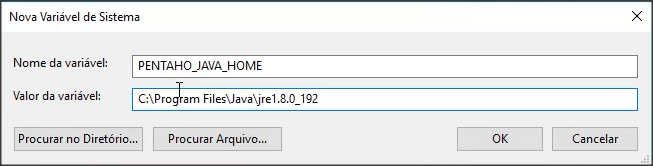
\includegraphics[scale=0.6]{Imagens/apendice variaveisambientepentahojavahome.png}
	\end{center}
	\legend{Fonte: Autor (2021).}
\end{figure}

\subsection{Instalação do PostgreSQL}
Execute o instalador e siga o assistente com a instalação padrão até o fim. A \autoref{apend_instalacaopostgres} apresenta uma captura de tela da janela de instalação do PostgreSQL.

\begin{figure}[htb]
	\caption{\label{apend_instalacaopostgres}Captura de tela da instalação do PostgreSQL.}
	\begin{center}
	    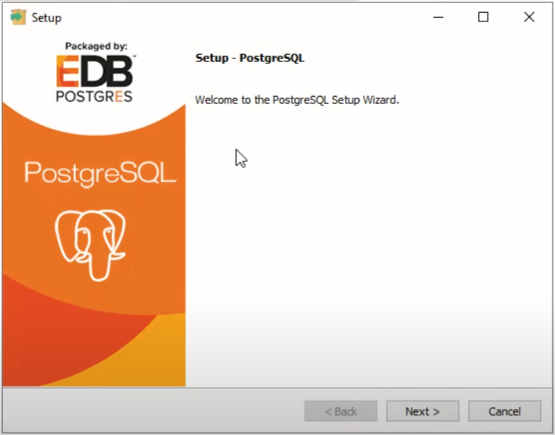
\includegraphics[scale=0.7]{Imagens/apendice postgres.png}
	\end{center}
	\legend{Fonte: Autor (2021).}
\end{figure}

\subsection{Instalação do SQL Power Architect}
Para instalar o SQL \textit{Power Architect}, execute o instalador, seguindo os passos da instalação padrão até o fim. Atenção ao selecionar a pasta de instalação, pois para utilizar o programa será necessário executar o arquivo \textbf{architect.exe}. A sugestão é adicionar um atalho em local de fácil acesso, visto que o programa por padrão não cria atalhos na área de trabalho. A \autoref{apend_sqlpower} apresenta uma captura de tela da janela de instalação do SQL Power Architect.

\begin{figure}[htb]
	\caption{\label{apend_sqlpower}Captura de tela da instalação do PostgreSQL.}
	\begin{center}
	    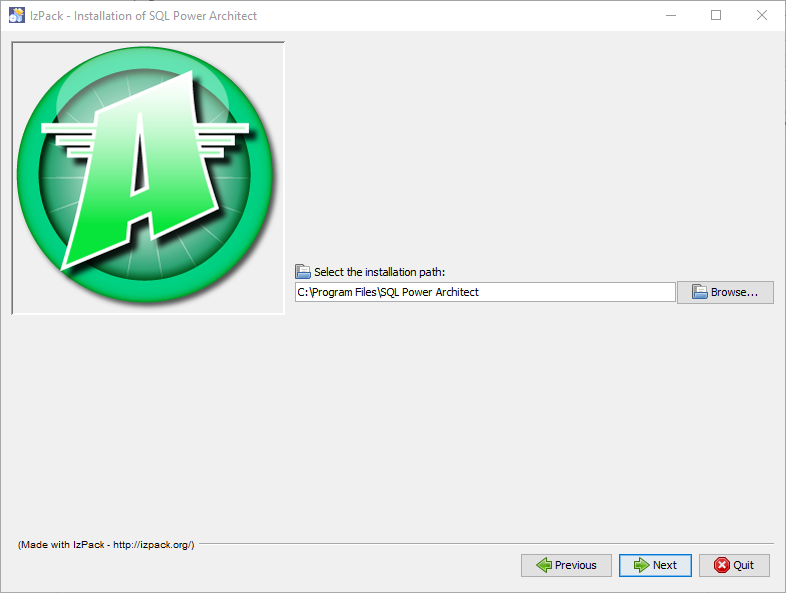
\includegraphics[scale=0.6]{Imagens/apendice instalacaopowersql.png}
	\end{center}
	\legend{Fonte: Autor (2021).}
\end{figure}

\section{Instalação do pacote Pentaho}
Vamos agora a instalação dos \textit{softwares} do pacote Pentaho. Crie uma pasta com o nome \textbf{Pentaho} na raiz do disco local C.

\subsection{Instalação do Pentaho \textit{Server}}
Copie o arquivo \textbf{pentaho-server-ce-9.1.0.0-324.zip} para o diretório \textbf{C: -> Pentaho} e descompacte-o. Em \textbf{C: -> Pentaho -> pentaho-server} abra o arquivo \textbf{start-pentaho.bat} e edite o parâmetro CATALINA\_OPTS, deixando-o da seguinte forma: "CATALINA\_OPTS=-Xms2048m -Xmx6144m". Esses valores correspondem a memória utilizada pelo servidor Apache incluso no \textit{Pentaho Server}, observe e respeite os limites de \textit{hardware} disponíveis. Também é uma boa prática adicionar um atalho para o arquivo \textbf{start-pentaho.bat} em local de fácil acesso, visto que o programa por padrão não cria atalhos na área de trabalho.

\subsection{Instalação do Pentaho \textit{Data Integration}}
Copie o arquivo \textbf{pdi-ce-9.1.0.0-324.zip} para \textbf{C: - Pentaho -> designer-tools} (crie esse diretório) e descompacte-o. Em \textbf{C: -> Pentaho -> designer-tools -> data-integration}, edite o arquivo \textbf{Spoon.bat} e na definição da variável PENTAHO\_DI\_JAVA\_OPTIONS, configure o tamanho da memória a ser utilizada da seguinte forma: "PENTAHO\_DI\_JAVA\_OPTIONS=-Xms1024m -Xms2048m -XX:MaxPermSize=256m". Observe e respeite os limites de \textit{hardware} disponíveis. É uma boa prática adicionar um atalho para o arquivo \textbf{Spoon.bat} em local de fácil acesso, visto que o programa por padrão não cria atalhos na área de trabalho.

\subsection{Instalação do Pentaho \textit{Report Designer}}
Copie o arquivo \textbf{prd-ce-9.1.0.0-324.zip} para \textbf{C: - Pentaho -> designer-tools} e descompacte-o. Em \textbf{C: -> Pentaho -> designer-tools -> report-designer}, edite o arquivo \textbf{report-designer.bat} e na linha 36 - \textbf{start Pentaho Report Designer "\%\_PENTAHO\_JAVA"}, configure o tamanho da memória a ser utilizada da seguinte forma: "-Xms1024m -Xms2048m -XX:MaxPermSize=256m". Observe e respeite os limites de \textit{hardware} disponíveis.

\subsection{Instalação do Pentaho \textit{Schema Workbench}}
Copie o arquivo \textbf{psw-ce-9.1.0.0-324.zip} para \textbf{C: - Pentaho -> designer-tools} e descompacte-o. Em \textbf{C: -> Pentaho -> designer-tools -> schema-workbench}, edite o arquivo \textbf{workbench.bat} e na linha 40 - \textbf{"\%\_PENTAHO\_JAVA"}, configure o tamanho da memória a ser utilizada da seguinte forma: "-Xms1024m -Xms2048m -cp". Observe e respeite os limites de \textit{hardware} disponíveis.

Para concluir, copie o arquivo do Driver PostgreSQL para Java, \textbf{postgresql-42.2.19.jar}, para os diretórios:
\begin{itemize}
   \item \textbf{C: -> Pentaho -> pentaho-server -> tomcat-lib};
   \item \textbf{C: -> Pentaho -> designer-tools -> data-integration -> lib};
   \item \textbf{C: -> Pentaho -> designer-tools -> report-designer -> lib -> jdbc}; 
   \item \textbf{C: -> Pentaho -> designer-tools -> schema-workbench -> drivers}.
\end{itemize}

% ---
\chapter{Orquestração dos Processos no Pentaho \textit{Data Integration}}
% ---

Com o Pentaho \textit{Data Integration} é possível determinar a execução de uma sequência lógica, não somente para atualização das dimensões, mas também para atualização das tabelas-fato. Para executar uma orquestração será necessário selecionar todos os processos de transformação, construindo um \textit{Job} de execução. As orquestrações podem executar várias transformações paralelamente e também podem ter execução agendada e periódica.

Para criar um \textit{Job} para executar as transformações, no Pentaho \textit{Data Integration}, clique no \textbf{\textit{Menu File -> New -> Job}}. As funcionalidades no Menu lateral esquerdo, são específicas para \textit{Jobs}. A \textit{step} que inicia uma orquestração e pode ser configurada para executar a partir de agendamentos está no pacote \textit{\textbf{General}, step \textbf{Start}}, como mostra a \autoref{apend_startjob}.

\begin{figure}[htb]
	\caption{\label{apend_startjob}Captura de tela da caixa de diálogo \textit{Start} no Pentaho PDI.}
	\begin{center}
	    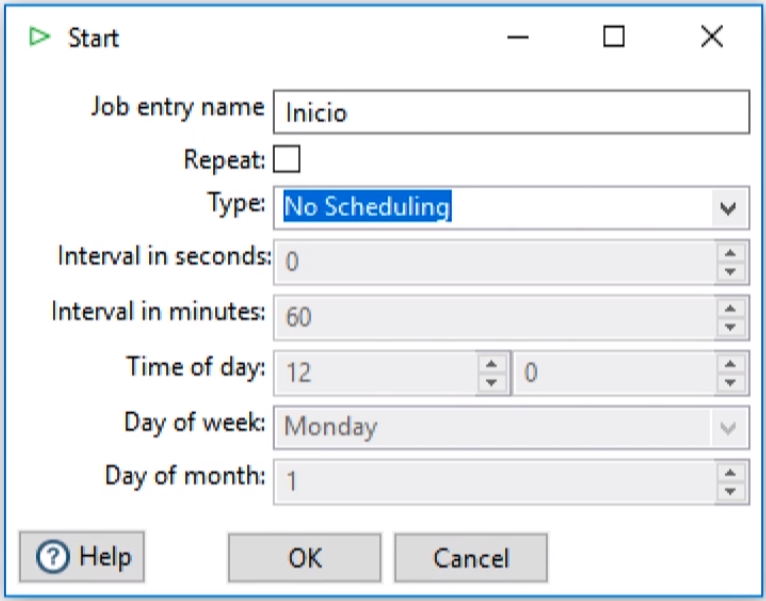
\includegraphics[scale=0.5]{Imagens/apendice startjobs shedule.png}
	\end{center}
	\legend{Fonte: Autor (2021).}
\end{figure}

Ainda no pacote \textit{\textbf{General}}, com a \textit{step \textbf{Transformation}} é possível escolher uma transformação para executar de acordo com a sequência estruturada.

\newpage
Além da orquestração de transformações, é possível ainda configurar a execução de \textit{Jobs} dentro de \textit{Jobs}, manipular e transferir arquivos e trabalhar com disparos de mensagens de \textit{e-mail}, como por exemplo, para situações de processo concluídos com sucesso e casos falhas na execução. Um exemplo de \textit{Job} com as opções citadas é apresentado pela \autoref{apend_stepsjobs}.

\begin{figure}[htb]
	\caption{\label{apend_stepsjobs}Exemplo de processos orquestrados no Pentaho PDI.}
	\begin{center}
	    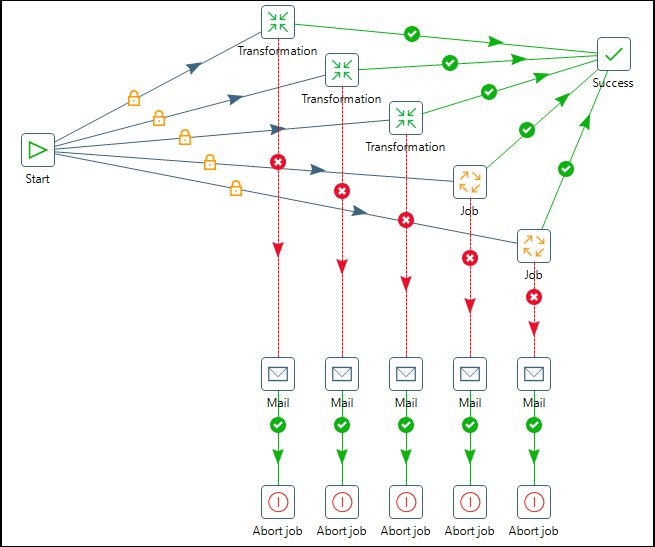
\includegraphics[scale=0.7]{Imagens/apendice jobs no pdi.png}
	\end{center}
	\legend{Fonte: Autor (2021).}
\end{figure}

Na versão Pentaho \textit{Community} não existe um servidor de "\textit{Sheduling}". Para usar as tarefas agendadas, o \textit{Spoon} do Pentaho \textit{Data Integration} deve permanecer em execução no servidor para disparar as tarefas.

\end{apendicesenv}